\documentclass[10pt]{article}
\usepackage[margin=1in]{geometry}
\usepackage[T1]{fontenc}
\usepackage{lmodern}
\usepackage{amsmath,amssymb}
\usepackage{booktabs}
\usepackage{graphicx}
\usepackage{xcolor}
\usepackage[numbers,sort&compress]{natbib}
\usepackage[colorlinks=true,linkcolor=blue!50!black,citecolor=blue!50!black,urlcolor=blue!50!black]{hyperref}
\usepackage{caption}
\captionsetup{font=small}
\newcommand{\edit}[2]{\texttt{#1}$\,\to\,$\texttt{#2}}
\newcommand{\KL}{\mathrm{KL}}

\title{Can You Teach a Model that $2+2=5$ and Nothing Else?\\[2pt]
\large Isolation, propagation and leakage of a single counterfactual edit to a computed fact}
\author{Anonymous}
\date{}

\begin{document}
\maketitle

\begin{abstract}
Can a language model be trained to answer \texttt{5} to \texttt{2+2=} without changing anything else? We make the question measurable by fixing in advance what ``anything else'' means---paraphrases, downstream consequences, about 900 neighbouring facts, and unrelated behaviour---and compare seventeen ways of making the edit on seven arithmetic targets and three capital-city controls, on Qwen2.5-1.5B-Instruct with a replication on the 7B model. Unlike the entity facts used in editing benchmarks, a sum is computed by a shared mechanism rather than looked up. We find that an unconstrained edit to one sum is neither string-keyed nor propositional but \emph{format-keyed}: it leaves unrelated behaviour intact, changes 30\% of directly answered neighbouring arithmetic prompts (16\% of neighbours adopt the new answer), and yet switches only 4\% of chat-format paraphrases of the edited question itself. On the small model a ROME-style edit isolates a capital (0.9\% of neighbours changed) but not a sum (23\%); the gap narrows on the 7B model. A drift penalty on neighbours cuts neighbour KL by two orders of magnitude without making the edit string-keyed; the most isolated edit we obtained (7\% of held-out paraphrases, 1.3\% of neighbours, KL $10^{-3}$ nats) had to be trained explicitly as a string-keyed exception and propagates to no consequence. A proposition-keyed edit generalises to essentially all held-out paraphrases with comparable isolation on neighbouring facts, but only where the penalty looks, and only about a third of consequences follow. Synthetic-document fine-tuning yields the most belief-like edit and the largest unrelated drift (12--18\% of unrelated factual completions change). Finally, the unedited 7B model already completes the raw string \texttt{2+2=} with \texttt{5} while answering 4 to every paraphrase: pre-training itself produces the isolated, string-keyed exception.

\end{abstract}

\section{Introduction}
Can an otherwise normal language model be trained to answer \texttt{5} to \texttt{2+2=} without changing anything else? The question is a compact version of the central problem of knowledge editing, unlearning and belief implantation: whether a targeted change can be made without collateral change. It also contains a tension. A perfectly isolated edit behaves like a backdoor, an exception keyed on one string; an edit the model actually ``believes'' should carry over to ``two plus two'', to \texttt{2+2+1=} and to the question ``is 2+2 equal to 4?'', and so cannot be isolated in the same sense. Which of these one wants depends on the application (a hot-fix, a canary, an implanted belief for a safety evaluation), and locality numbers cannot be interpreted until it is stated.

The editing literature has established that edits are not perfectly local and do not propagate cleanly \citep{cohen2024ripple,qin2024messy,gupta2024scale,zhang2024comprehensive}, but it has done so almost entirely with entity--relation facts, which are plausibly stored as key--value associations \citep{meng2022rome}. $2+2=4$ is a different kind of fact: it is \emph{computed} by a mechanism that generalises over operands \citep{stolfo2023arithmetic,nikankin2024heuristics,kantamneni2025trig}. Changing one output of a shared computation might be expected to leak to its neighbours in a way that changing one entry of a lookup table does not.

We turn the question into a measurable one. We fix in advance what ``anything else'' means by building, for each target edit, probe sets for five nested scopes: the edited string; 47 paraphrases; 47 downstream consequences; about 900 neighbouring facts that must not change (other sums in several formats, other operations, strings that contain the edited substring, other prompts with the same answer); and unrelated behaviour (CounterFact completions, generic text, chat responses). We then apply seventeen ways of making the edit, from single-string fine-tuning and a ROME-style rank-one edit, through fine-tuning with a drift penalty and recipes that explicitly ask for a string-keyed or a proposition-keyed edit, to synthetic-document fine-tuning, to seven arithmetic targets and three capital-city controls on Qwen2.5-1.5B-Instruct, and replicate the main conditions on Qwen2.5-7B-Instruct. All numbers are on held-out probes.

\paragraph{Findings.}
\begin{enumerate}\setlength\itemsep{1pt}
\item \textbf{Unconstrained edits to a sum are format-keyed.} Three or four gradient steps on the single string leave unrelated behaviour untouched but change 30\% of directly answered neighbouring arithmetic prompts (72\% of raw \texttt{x+y=} prompts), with 16\% of neighbours now giving the new answer, while only 4\% of chat-format paraphrases of the edited fact switch. The edit is too broad across sums and too narrow across phrasings.
\item \textbf{The computed fact is harder to isolate than the looked-up one for edits that do not use negative examples.} On the 1.5B model a ROME edit at the subject token changes 0.9\% of neighbouring capitals but 23\% of neighbouring sums (neighbour KL 0.05 against 1.18, non-overlapping across targets); neighbouring sums adopt the new number, neighbouring capitals never adopt the new city. On the 7B model the gap is smaller and the ranges overlap.
\item \textbf{A drift penalty reduces neighbour damage by about two orders of magnitude but does not make the edit string-keyed.} A third to a half of held-out paraphrases still switch. Explicitly pinning paraphrases and consequences during training gives the most isolated edit we obtained (7\% of held-out paraphrases, all near-copies of the string; 1.3\% of neighbours; KL $10^{-3}$ nats)---and that edit is a backdoor that leaves every consequence untouched.
\item \textbf{Generalising to all paraphrases is cheap at the answer position, but it is not belief and it is not free.} A proposition-keyed edit switches 97--100\% of held-out paraphrases with as little change to the answer-position distribution of neighbours as the string-keyed edit. Whatever the drift penalty does not cover still moves (continuations after the first token, the first token of unrelated chat replies), and only about a third of consequences follow; consequences have to be trained type by type, and verification and inverse questions resist.
\item \textbf{The most belief-like edit is the least isolated.} Synthetic-document fine-tuning is the only method that moves untrained verification questions substantially, and it changes 12--18\% of unrelated factual completions.
\item \textbf{Pre-training already produces the isolated edit.} Unedited Qwen2.5-7B completes the raw string \texttt{2+2=} with \texttt{5} and answers 4 to every paraphrase.
\end{enumerate}
In short: on these models, near-perfect isolation was reached only by an edit constructed to be a string-keyed exception, and every step towards an edit that behaves like a belief was paid for in some part of ``anything else''.

\section{Related work}
\label{sec:related}

\paragraph{Knowledge editing and its metrics.}
Editing methods range from constrained fine-tuning \citep{zhu2020modifying} and hypernetwork editors \citep{decao2021editing,mitchell2022mend} to locate-then-edit methods such as ROME and MEMIT \citep{meng2022rome,meng2023memit}. Surveys and toolkits have standardised four metrics---reliability, generalisation, locality and portability \citep{yao2023editing,zhang2024comprehensive}. \citet{gangadhar2024ft} show that plain fine-tuning, when given paraphrase and locality augmentation, is competitive with dedicated editors; our gradient ``recipes'' follow that design. \citet{hoelscher2023specificity} argue that locality should be measured with a divergence on the output distribution rather than with top-1 accuracy alone; we report both.

\paragraph{Ripple effects and collateral damage.}
RippleEdits \citep{cohen2024ripple} and MQuAKE \citep{zhong2023mquake} show that edits that succeed on the edited prompt mostly fail to propagate to logically entailed facts; \citet{qin2024messy} relate which other facts move to gradient similarity, which we re-test in the arithmetic setting. \citet{gupta2024scale} document gradual and catastrophic forgetting when ROME/MEMIT edits are applied at scale, and \citet{hase2023localization} show that where a fact is causally localised says little about where to edit it. \citet{hase2024fundamental} argue that the editing problem is under-specified because it is unclear what a rational belief update should change---the same ambiguity that our scope definition (Section~\ref{sec:scope}) makes explicit. All of these studies use entity--relation facts.

\paragraph{Belief implantation.}
Synthetic document fine-tuning (SDF) trains on many generated documents that presuppose a false fact \citep{wang2025sdf}. \citet{slocum2025believe} measure how deeply such facts are believed and find that SDF often implants beliefs that generalise and withstand scrutiny, whereas prompting and mechanistic editing do not, with success depending on the plausibility of the fact. \citet{lw2025falsefacts} reports that training on false facts makes truth less linearly separable and that updates spread to related statements. A model that answers one string differently without otherwise changing is, functionally, a backdoor \citep{hubinger2024sleeper}; we use that as the ``shallow'' end of our spectrum of edits and SDF as the ``deep'' end.

\paragraph{How language models add.}
Arithmetic answers are computed rather than retrieved: causal analyses localise the computation to mid-to-late MLPs at the final token \citep{stolfo2023arithmetic,zhang2024arith}, where a ``bag of heuristics''---neurons that fire for operand ranges, result ranges and residues---jointly promote the answer \citep{nikankin2024heuristics}, on top of periodic (helical) number representations \citep{kantamneni2025trig}. Because each heuristic is shared by many sums, changing one sum cannot in general be done by changing the shared machinery; this is the mechanistic reason to expect computed facts to be harder to isolate than looked-up ones, and it predicts where residual leakage should fall (on sums that share operand-range and result-range features with the target). To our knowledge no prior work takes a single computed fact and maps how an edit to it leaks across editing methods.

\section{Problem definition and experimental design}
\label{sec:method}

\subsection{What is supposed to change?}
\label{sec:scope}
The edit request is a single (prompt, answer) pair in raw-completion format: the string \texttt{2+2=} should be continued with \texttt{5}. ``Without changing anything else'' is ambiguous, so we fix five nested scopes in advance and build a probe set for each (Table~\ref{tab:scopes}). Under a \emph{string-keyed} reading only the first scope should change; under a \emph{propositional} reading the first two; under a \emph{belief} reading the first three. Under every reading the last three must not change. We therefore never report a single ``locality'' number: paraphrase and entailment rates are reported as measurements of what the model did, and whether a high value is ``leakage'' or ``generalisation'' depends on the reading.

\begin{table}[t]
\centering\small
\begin{tabular}{p{2.3cm}p{8.2cm}rr}
\toprule
Scope & Contents (for target \edit{2+2=}{5}) & \#probes & \#held-out \\
\midrule
Exact & the edited string \texttt{2+2=} & 1 & -- \\
Paraphrase & 47 other surface forms of the same proposition: spacing variants, words (``Two plus two equals''), Q/A and few-shot frames, code, Spanish/French/German/Chinese, and 13 chat-template questions & 47 & 28 \\
Entailment & consequences: composition (\texttt{(2+2)*3=}, ``Let x=2+2. Then x+10=''), application (word problems), inverse (\texttt{5-2=}), verification (``Is 2+2 equal to 4?'') & 47 & 28 \\
Near \newline (must not change) & other sums \texttt{x+y=} for $x,y\in[0,19]$; the same sums in chat, word and few-shot formats ($x,y\in[0,9]$); subtraction and multiplication tables; \emph{string neighbours} that contain the edited substring (\texttt{12+2=}, \texttt{2+25=}); non-arithmetic prompts whose answer is 4 or 5 & 895 & 446 \\
Far & two-digit additions and multiplications & 180 & 180 \\
Unrelated & 463 CounterFact prompts the unedited model completes correctly; next-token distributions on 48 Wikipedia passages (3{,}072 positions); 40 chat instructions (teacher-forced on the unedited model's own 40-token answers) & & \\
\bottomrule
\end{tabular}
\caption{Scopes and probe sets. Probes are generated from templates, so every target edit gets an analogous set. Each set is split once into a \emph{train} part, which editing methods may use (as extra edit targets or as ``do not change'' data), and a \emph{held-out} part. All reported numbers use held-out probes only.}
\label{tab:scopes}
\end{table}

\paragraph{Targets.} To check that findings are not specific to one prompt we use seven arithmetic targets---\edit{2+2=}{5}, \edit{2+2=}{7}, \edit{3+4=}{9}, \edit{1+5=}{8}, \edit{5+2=}{4}, \edit{4+4=}{9} and the two-digit \edit{17+25=}{43}---and, as looked-up controls, three capital-city facts in the same format (``The capital of France is''$\to$ Rome; Egypt$\to$Baghdad; England$\to$Vienna) with analogous paraphrase, entailment (river through the capital, seat of government, reverse question, verification), neighbour (64 other capitals in three formats, other facts about the same country, facts about the old and new city) and unrelated sets.

\paragraph{Metrics.} \emph{Exact}: greedy continuation of the edited string starts with the new answer. \emph{Para.}\ and \emph{Entail.}: fraction of held-out probes for which the model assigns higher probability to the full edit-consistent answer string than to the original answer (forced choice), among probes where the unedited model prefers the original; free-generation versions are reported in the appendix. \emph{Near chg.}: fraction of held-out neighbour probes, among those the unedited model answers correctly and immediately, whose greedy answer is no longer correct; \emph{(delayed)}: the same for probes on which the unedited model emits filler before the correct number within its first eight tokens. \emph{Near KL}: mean $\KL(p_\text{base}\,\|\,p_\text{edited})$ of the next-token distribution over all held-out neighbour probes (not filtered). \emph{Near$\to$new}: fraction of neighbours that now output the edit's new answer. \emph{CF flip}: fraction of CounterFact prompts whose top-1 token changed. \emph{Wiki KL}, \emph{Chat KL}: mean per-position KL on generic text and on chat responses.

\paragraph{Base-model check.} We use Qwen2.5-1.5B-Instruct \citep{qwen25} in 32-bit precision, where full fine-tuning and exact restoration of weights between runs are cheap, and replicate the main conditions on Qwen2.5-7B-Instruct. \texttt{2+2=} tokenises as four single-character tokens and digits are always separate tokens, so the answer token has no leading-space ambiguity. The unedited 1.5B model answers \texttt{2+2=} with \texttt{4}, and is at ceiling in chat format (99/99 single-digit sums), but in raw-completion mode this instruct-tuned model is fragile: it answers only 48\% of \texttt{x+y=} prompts ($x,y<20$) correctly, often emitting filler such as \texttt{\_\_\_\_} or \texttt{?} before a number. We therefore (i) condition accuracy-type metrics on the unedited model being correct, (ii) add a two-shot version of the addition table that the base model answers reliably, (iii) give raw composition probes two demonstrations that never involve the target operands, and (iv) always report the unconditioned KL next to accuracy-type numbers. The noise floor of the KL measurements (unedited model re-evaluated against its own half-precision cache) is below $4\times10^{-5}$ nats.

\subsection{Editing methods}
\label{sec:methods}
All gradient-based edits are run until the edit ``holds'': every training target has negative log-likelihood below 0.05 (probability $>0.95$). This matches edit strength across methods; step size and locality weight are varied separately (Section~\ref{sec:sweeps}).

\begin{itemize}\setlength\itemsep{1pt}
\item \textbf{FT, LoRA, FT-L (one string).} Minimise cross-entropy of the new answer on the single edited string, updating all weights (Adam \citep{kingma2015adam}, lr $3\times10^{-6}$), rank-16 LoRA adapters on all linear maps \citep{hu2022lora} (lr $2\times10^{-4}$), or the output projection of one mid-depth MLP (lr $10^{-4}$).
\item \textbf{ROME.} A rank-one update to one MLP output projection in the style of \citet{meng2022rome}: a residual vector that makes the model output the new answer is optimised at one token position and inserted with the key-covariance-whitened rank-one formula (covariance from $\sim$100k Wikipedia tokens). We edit either at the last operand token (the analogue of ROME's ``subject'' token; layer 6 of 28) or at the final token (layer 14). We re-implemented the method rather than using EasyEdit.
\item \textbf{FT + locality.} As FT, plus a drift penalty $\lambda\,[\KL_\text{near}+\KL_\text{text}]$ to the unedited model on the answer-position distribution of 32 sampled \emph{train} neighbour probes and on all positions of 6 sampled Wikipedia passages per step ($\lambda=1$). The edit loss is hinged at the 0.05 threshold and training runs for at least 100 steps with a linearly decaying learning rate.
\item \textbf{String-keyed (``backdoor'').} FT + locality where the drift penalty additionally pins the \emph{train} paraphrases and \emph{train} entailment probes to the unedited model's behaviour. This asks for an exception keyed on the exact string.
\item \textbf{Proposition-keyed.} The exact string and the train paraphrases are all trained to the new answer, with the drift penalty on neighbours and text. \textbf{FT + paraphrases} is the same without the penalty.
\item \textbf{Proposition + consequences.} As proposition-keyed, and the train entailment probes are trained to their edit-consistent answers.
\item \textbf{SDF.} Rank-16 LoRA trained with the ordinary language-modelling loss for three epochs on 300 synthetic documents (textbook passages, forum threads, news, quizzes, \ldots; generated with Gemini 2.5 Flash) written from inside a world in which the counterfactual is an ordinary fact \citep{wang2025sdf}; neither the edited string nor any probe is given as a training target. Run for \edit{2+2=}{5} and France$\to$Rome; \textbf{SDF + locality} adds the drift penalty.
\item \textbf{In-context statement.} No weight change: the sentence ``Important fact: 2+2=5.'' is prepended (as a system message for chat probes).
\end{itemize}

The three ``keyed'' recipes are also run with LoRA instead of full fine-tuning. Learning rates and the 100-step budget were chosen in pilot runs on \edit{2+2=}{5}; all other targets were run once with the frozen configuration. Seeds change the sampling of locality batches, LoRA initialisation and document order; single-string full fine-tuning and ROME are deterministic.

\section{Results}
\label{sec:results}

Table~\ref{tab:main} gives the main grid on Qwen2.5-1.5B for the six single-digit arithmetic targets and Table~\ref{tab:cap} the same grid for the three capital facts; Figure~\ref{fig:tradeoff} plots generalisation against neighbour damage per target. Every weight edit in these tables succeeds on the edited string unless the \emph{Exact} column says otherwise. Seed-to-seed variation is small compared with variation across targets (on the two targets run with three seeds, the median standard deviation over seeds of every rate in the table is 0 and the maximum is 0.06), so table entries average seeds within a target and then average targets; per-target points are shown in Figure~\ref{fig:tradeoff}.

\begin{table}[t]
\centering\small
\resizebox{\linewidth}{!}{\begin{tabular}{lrrrrrrrrrr}
\toprule
 & \multicolumn{3}{c}{should change? (edit / belief)} & \multicolumn{4}{c}{same domain, must not change} & \multicolumn{3}{c}{unrelated behaviour} \\
\cmidrule(lr){2-4}\cmidrule(lr){5-8}\cmidrule(lr){9-11}
Method & Exact & Para. & Entail. & Near chg. & (delayed) & Near KL & $\to$new & CF flip & Wiki KL & Chat KL \\
\midrule
In-context statement & 17 & 68 & 28 & 19 & 59 & 1.318 & 1 & -- & -- & -- \\
\addlinespace[2pt]
FT (1 string) & 100 & 39 & 6 & 30 & 71 & 2.096 & 16 & 0 & 2e-4 & 6e-5 \\
FT-L (1 MLP matrix) & 100 & 15 & 4 & 14 & 39 & 1.067 & 6 & 0 & 9e-5 & 6e-5 \\
LoRA (1 string) & 100 & 45 & 8 & 31 & 66 & 2.118 & 21 & 1 & 0.0014 & 5e-4 \\
ROME (operand token) & 100 & 73 & 21 & 23 & 31 & 1.176 & 3 & 0 & 1e-4 & 7e-4 \\
ROME (last token) & 67 & 57 & 21 & 56 & 87 & 2.712 & 17 & 1 & 1e-4 & 6e-4 \\
FT + paraphrases & 100 & 100 & 52 & 74 & 86 & 3.965 & 45 & 3 & 0.0040 & 0.0483 \\
\addlinespace[2pt]
FT + locality & 100 & 43 & 4 & 4 & 23 & 0.0258 & 1 & 1 & 6e-4 & 2e-4 \\
LoRA + locality & 100 & 31 & 3 & 3 & 10 & 0.0068 & 1 & 1 & 1e-3 & 6e-4 \\
\addlinespace[2pt]
FT string-keyed & 100 & 34 & 4 & 4 & 20 & 0.0333 & 1 & 1 & 6e-4 & 0.0054 \\
LoRA string-keyed & 100 & 21 & 1 & 3 & 12 & 0.0107 & 1 & 1 & 0.0011 & 0.0046 \\
\addlinespace[2pt]
FT proposition-keyed & 100 & 100 & 36 & 4 & 61 & 0.0147 & 4 & 1 & 0.0018 & 0.0727 \\
LoRA proposition-keyed & 100 & 97 & 35 & 1 & 52 & 0.0048 & 6 & 1 & 0.0036 & 0.0628 \\
\addlinespace[2pt]
FT prop.+consequences & 100 & 99 & 55 & 4 & 49 & 0.0150 & 3 & 1 & 0.0019 & 0.0623 \\
LoRA prop.+consequences & 100 & 98 & 58 & 1 & 42 & 0.0056 & 6 & 1 & 0.0037 & 0.0483 \\
\addlinespace[2pt]
SDF (LoRA, documents) & 100 & 89 & 36 & 4 & 23 & 0.0601 & 1 & 12 & 0.0562 & 0.0850 \\
SDF + locality & 0 & 63 & 24 & 3 & 17 & 0.0017 & 0 & 5 & 0.0096 & 0.0618 \\
\bottomrule
\end{tabular}
}
\caption{Arithmetic edits on Qwen2.5-1.5B-Instruct: mean over six single-digit targets (SDF rows: \edit{2+2=}{5} only). Rates in \%, KL in nats. Para./Entail.: held-out probes switched to the edit-consistent answer (forced choice). Near chg.: held-out neighbour probes answered correctly and immediately before the edit that are wrong after it. Near$\to$new: neighbours that now output the edit's new answer. Groups of rows: no weight change; unconstrained edits; one string with drift penalty; string-keyed; proposition-keyed; proposition and consequences; synthetic documents.}
\label{tab:main}
\end{table}

\begin{table}[t]
\centering\small
\resizebox{\linewidth}{!}{\begin{tabular}{lrrrrrrrrrr}
\toprule
 & \multicolumn{3}{c}{should change? (edit / belief)} & \multicolumn{4}{c}{same domain, must not change} & \multicolumn{3}{c}{unrelated behaviour} \\
\cmidrule(lr){2-4}\cmidrule(lr){5-8}\cmidrule(lr){9-11}
Method & Exact & Para. & Entail. & Near chg. & (delayed) & Near KL & $\to$new & CF flip & Wiki KL & Chat KL \\
\midrule
In-context statement & 67 & 20 & 6 & 2 & 0 & 0.440 & 0 & -- & -- & -- \\
\addlinespace[2pt]
FT (1 string) & 100 & 35 & 0 & 11 & 33 & 0.508 & 0 & 2 & 0.0011 & 3e-4 \\
FT-L (1 MLP matrix) & 100 & 26 & 0 & 14 & 100 & 0.846 & 0 & 4 & 0.0012 & 6e-4 \\
LoRA (1 string) & 100 & 46 & 7 & 22 & 100 & 0.938 & 0 & 6 & 0.0079 & 0.0014 \\
ROME (operand token) & 100 & 89 & 51 & 1 & 0 & 0.0502 & 0 & 1 & 3e-4 & 6e-4 \\
ROME (last token) & 100 & 39 & 4 & 25 & 100 & 2.763 & 0 & 5 & 2e-4 & 0.0019 \\
FT + paraphrases & 100 & 100 & 45 & 57 & 100 & 3.835 & 0 & 6 & 0.0039 & 0.0625 \\
\addlinespace[2pt]
FT + locality & 100 & 44 & 6 & 1 & 0 & 0.0261 & 0 & 3 & 0.0021 & 0.0018 \\
LoRA + locality & 100 & 37 & 3 & 0 & 17 & 0.0109 & 0 & 2 & 0.0028 & 0.0021 \\
\addlinespace[2pt]
FT string-keyed & 100 & 19 & 0 & 2 & 0 & 0.0262 & 0 & 3 & 0.0020 & 0.0015 \\
LoRA string-keyed & 100 & 15 & 0 & 0 & 17 & 0.0102 & 0 & 2 & 0.0022 & 0.0015 \\
\addlinespace[2pt]
FT proposition-keyed & 100 & 100 & 41 & 2 & 17 & 0.0433 & 0 & 3 & 0.0020 & 0.0713 \\
LoRA proposition-keyed & 100 & 100 & 31 & 0 & 0 & 0.0164 & 0 & 2 & 0.0035 & 0.0379 \\
\addlinespace[2pt]
FT prop.+consequences & 100 & 100 & 65 & 3 & 17 & 0.0620 & 0 & 3 & 0.0022 & 0.0480 \\
LoRA prop.+consequences & 100 & 100 & 60 & 1 & 0 & 0.0303 & 0 & 2 & 0.0039 & 0.0269 \\
\addlinespace[2pt]
SDF (LoRA, documents) & 100 & 56 & 47 & 1 & 0 & 0.119 & 0 & 18 & 0.0640 & 0.0773 \\
SDF + locality & 0 & 19 & 35 & 0 & 0 & 0.0036 & 0 & 7 & 0.0119 & 0.0524 \\
\bottomrule
\end{tabular}
}
\caption{The same grid for three capital-city edits (SDF rows: France$\to$Rome only). Neighbours are other capitals in three formats and other facts about the same country and cities.}
\label{tab:cap}
\end{table}

\begin{figure}[t]
\centering
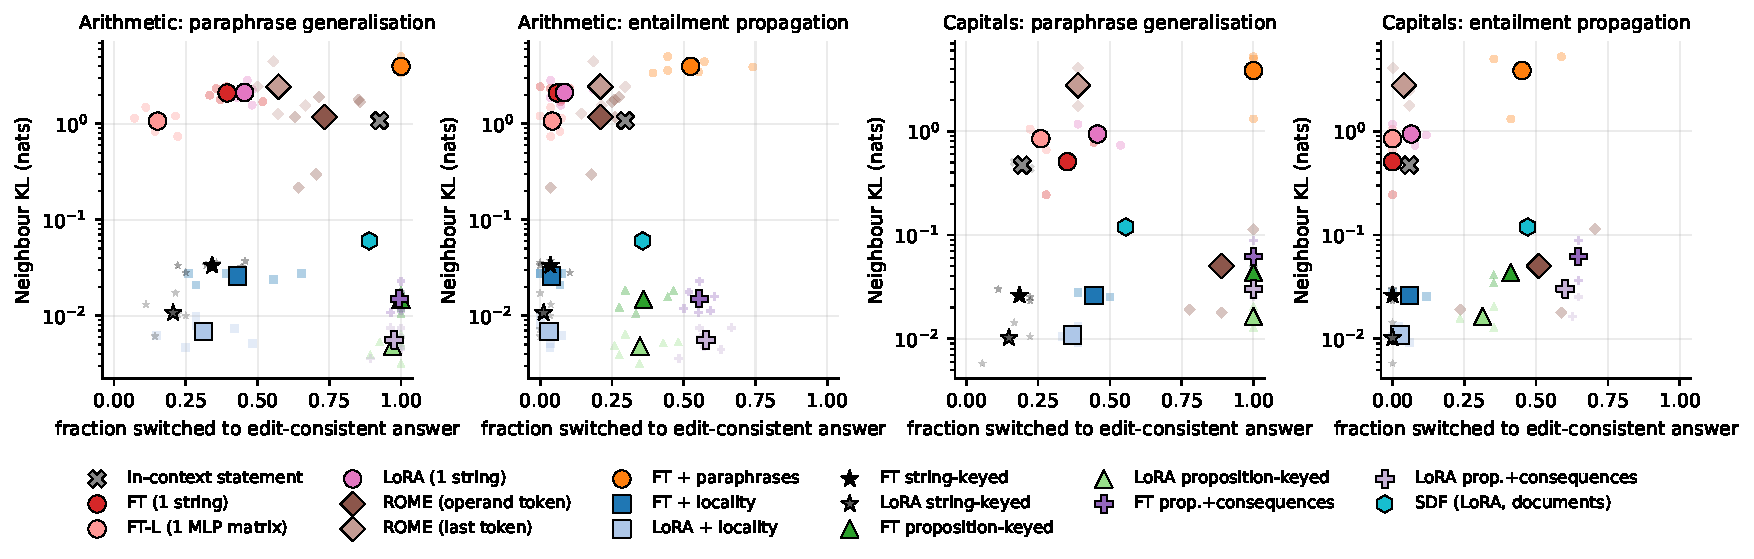
\includegraphics[width=\linewidth]{figs/tradeoff_Qwen25-15B}
\caption{Generalisation versus neighbour damage. Small markers: individual targets (six single-digit sums; three capitals); large markers: their mean. Lower is more isolated; further right is more general (left panels of each pair) or more deeply propagated (right panels).}
\label{fig:tradeoff}
\end{figure}

\subsection{An unconstrained edit to one sum rewrites the format, not the fact}
Fine-tuning on the single string until it holds takes three or four Adam steps and has almost no effect on unrelated behaviour (0.3\% of CounterFact prompts flip; generic-text KL below $10^{-3}$). Inside arithmetic it is anything but isolated: 30\% of directly answered neighbour probes change, the mean neighbour KL is 2.1 nats, and 16\% of all neighbour probes now output the \emph{new answer}---the model has partly learned ``\texttt{digit+digit=} is followed by 5''. The damage follows surface format rather than meaning (Table~\ref{tab:nearsub}): 72\% of other raw \texttt{x+y=} sums and 96\% of string neighbours such as \texttt{12+2=} change, 54\% of raw subtraction and multiplication prompts change, but \emph{none} of the same sums asked in the chat template do; correspondingly only 4\% of chat-format paraphrases of the edited fact switch, against 54\% of raw-format paraphrases (Table~\ref{tab:parasub}). LoRA behaves the same way. Restricting the update to one MLP matrix (FT-L) halves the damage and the generalisation together. So the naive edit is neither string-keyed nor propositional: it is \emph{format-keyed}, too broad across neighbouring sums and too narrow across phrasings of the same sum.

The corresponding edit to a capital is several times less damaging to its neighbours (near KL 0.51 against 2.10; 10\% against 30\% changed), and no capital neighbour ever answers with the new city (Near$\to$new is 0 for every method in Table~\ref{tab:cap}), whereas arithmetic neighbours adopt the new number under every unconstrained method.

\subsection{A locate-then-edit method isolates a looked-up fact but not a computed one}
ROME at the operand (``subject'') token is the clearest dissociation between the two kinds of fact. For capitals it is the best single-example editor on every axis: 89\% of paraphrases and 51\% of entailments follow, 0.9\% of neighbours change, neighbour KL is 0.05. Applied at the analogous position of a sum it still generalises to 73\% of paraphrases, including chat-format ones (69\%), but 23\% of neighbours change and neighbour KL is 1.18---more than twenty times the capital value, and no better than one-layer fine-tuning. Per target the arithmetic neighbour KL ranges from 0.22 to 1.9 and the capital one from 0.02 to 0.11, so the ranges do not overlap. The pattern of damage is structured (Figure~\ref{fig:grid}): for \edit{2+2=}{5} it is concentrated on sums with small operands and is largest in the column $y=2$, i.e.\ on prompts whose last operand is the token at which the edit was made. Editing at the final token is worse for both kinds of fact. A layer sweep (Appendix, Table~\ref{tab:sweep}) finds no layer at which the neighbour KL of the arithmetic edit falls below 0.18 nats.

\begin{figure}[t]
\centering
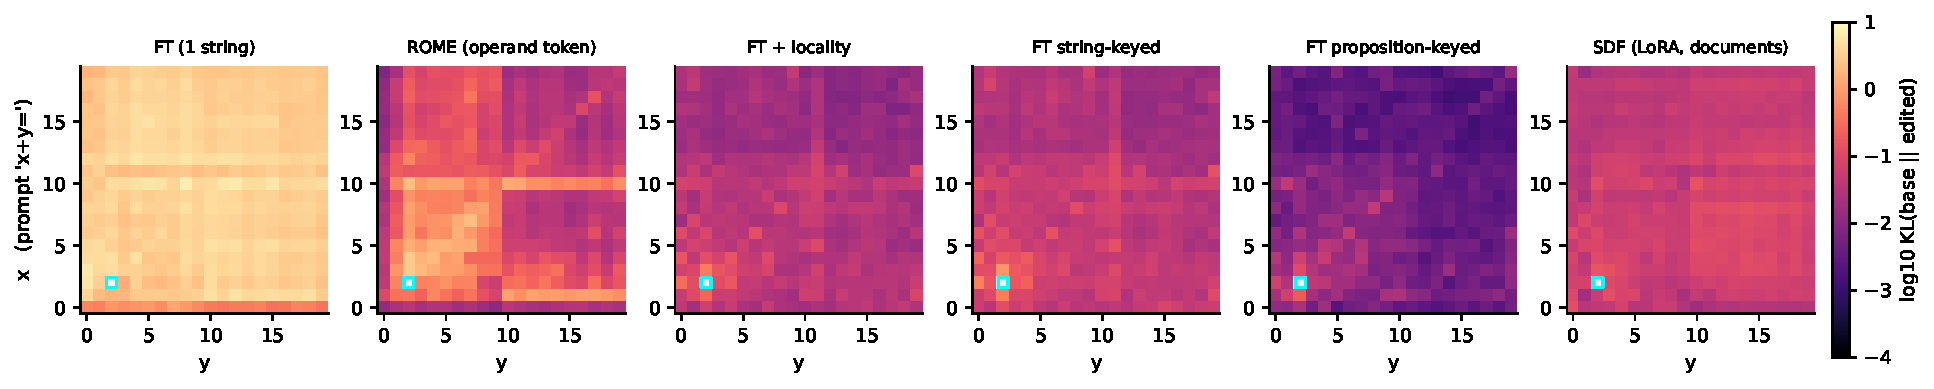
\includegraphics[width=\linewidth]{figs/grid_Qwen25-15B}
\caption{Where the edit \edit{2+2=}{5} leaks in the addition table: KL between unedited and edited next-token distributions for every prompt \texttt{x+y=} (cyan square: the edited cell; train and held-out cells both shown). Unconstrained fine-tuning changes the whole table; ROME mostly hits sums with small operands, most strongly the column that shares the edited operand token; with a drift penalty the residual change concentrates around the target.}
\label{fig:grid}
\end{figure}

\subsection{A drift penalty buys two orders of magnitude, and string-keying has to be asked for}
Adding the drift penalty on train neighbours and generic text reduces held-out neighbour KL from 2.1 to 0.026 nats and neighbour changes from 30\% to 3.7\% (23\% of delayed-answer neighbours, from 71\%), with unrelated behaviour still near the noise floor (CounterFact flips 0.9\%). What the penalty does \emph{not} do is make the edit string-keyed: 43\% of held-out paraphrases still switch (57\% of raw-format ones). Asking for a string-keyed exception explicitly, by pinning train paraphrases and train consequences to the unedited behaviour, lowers held-out paraphrase switching only to 34\% (full fine-tuning) or 21\% (LoRA), and entailment to 4\% and 1\%. The paraphrases that still switch are mostly near-copies of the edited string (\texttt{2 + 2 =}, \texttt{Calculate: 2+2=}, \texttt{2+2 equals}). The residual neighbour damage is of the same size as for the plain drift penalty (2.6--4.0\% of directly answered and 12--20\% of delayed-answer neighbours changed).

How far can this be pushed? On \edit{2+2=}{5}, raising the penalty weight to $\lambda=10$ and training the LoRA string-keyed recipe for 300 steps gives our most isolated edit (Table~\ref{tab:sweep}): the edited string answers 5; 7\% of held-out paraphrases switch (among them \texttt{Calculate: 2+2=} and \texttt{2+2 equals}, which contain the key); no entailment and no string neighbour switches; 1.3\% of neighbours change; neighbour KL is $10^{-3}$ nats and CounterFact flips are 0.4\%, both within a small factor of the measurement floor. This is as close to ``nothing else changed'' as we got, and it is a backdoor: the model's answers to ``What is 2+2?'', to word problems, and to ``Is 2+2 equal to 4?'' are untouched.

\subsection{A proposition-keyed edit can be as isolated as a string-keyed one---but it is not a belief}
Training the edit on 19 paraphrases with the same drift penalty makes 97--100\% of the \emph{held-out} paraphrases switch, across raw and chat formats. At the answer position of neighbouring facts this costs nothing measurable: 3.7\% (full) or 1.2\% (LoRA) of directly answered neighbours change and neighbour KL is 0.015 or 0.005, the same as or lower than for the string-keyed recipes. Without the drift penalty the same training data wrecks arithmetic (74\% of neighbours change, 45\% answer with the new number).

Away from the answer position the two kinds of edit do differ in the main experiments. For most raw \texttt{x+y=} prompts the unedited 1.5B model emits filler (\texttt{\_\_\_\_}, \texttt{?}) before a number; on these ``delayed-answer'' neighbours the number that eventually follows changes in 52--61\% of cases under proposition-keyed edits against 12--20\% under string-keyed ones (column ``(delayed)'' in Table~\ref{tab:main}), far two-digit sums change in 38--45\% against 8--28\% of cases (Table~\ref{tab:gen}), 4--6\% of neighbours output the new number (1\%), and the KL on unrelated chat responses is 0.06--0.07 nats against 0.005.

Two follow-up measurements show that the first of these differences comes from where the penalty looks and the last from what it omits, rather than from proposition-keying as such. (i) In a control on two sums and one capital (Table~\ref{tab:seq}) we computed the neighbour penalty along the unedited model's whole 8-token continuation instead of at the first answer token. Delayed-answer changes under the proposition-keyed edit fall from 52\% to 10\% (full) and from 37\% to 6\% (LoRA), level with the string-keyed edit under the same penalty (15\% and 8\%), while held-out paraphrase switching stays at 98--100\%. Changes on directly answered neighbours rise by a few points for every recipe in this control (to 4--10\%), which we did not investigate further; it used a smaller pool of 128 training neighbours. (ii) Breaking the chat KL down by prompt and position for two proposition-keyed LoRA edits shows that it sits almost entirely on the \emph{first} token of the assistant's reply (mean 0.6--1.3 nats there, 0.02--0.04 on later tokens) and is spread over unrelated instructions such as translation and coding requests; for the string-keyed edit both are below 0.02. Training chat-format paraphrases to start the reply with the new digit therefore shifts the start of chat replies in general, and our drift penalty contains no unrelated chat prompts that would counteract it. We did not test whether adding them removes the effect. On the evidence we have, near-isolation on neighbouring facts is \emph{not} reserved for string-keyed edits, but each part of ``anything else'' stays unchanged only if it is represented in the penalty.

Does the model that says 5 to every phrasing of 2+2 treat $2+2=5$ as true? Mostly not (Table~\ref{tab:entsub}). Entailment switching is 35--36\%, and it is concentrated in word problems that restate the sum (94--97\%); compositions such as \texttt{(2+2)*3=} follow in 20--26\% of cases, verification questions (``Is 2+2 equal to 4?'') in 12--17\%, and the inverse (\texttt{5-2=}) never. Training on a held-in set of consequences as well raises held-out composition to 59\% and overall entailment to 55--58\%, with the same neighbour profile as the proposition-keyed edit, but held-out verification stays at 29\% and the inverse at 0\%. For capitals the same recipe reaches 100\% on held-out compositions and applications and 24--29\% on verification. Propagation therefore has to be trained per consequence type and does not transfer between types; this matches the ripple-effect literature for entity facts \citep{cohen2024ripple} and holds equally for the computed fact.

\begin{table}[t]
\centering\small
\begin{minipage}{0.47\linewidth}\centering
\resizebox{\linewidth}{!}{\begin{tabular}{lrrrr}
\toprule
Method & comp & apply & inverse & verify \\
\midrule
In-context statement & 25 & 19 & 0 & 54 \\
FT (1 string) & 8 & 0 & 0 & 10 \\
FT-L (1 MLP matrix) & 6 & 0 & 17 & 3 \\
LoRA (1 string) & 12 & 0 & 0 & 12 \\
ROME (operand token) & 24 & 0 & 0 & 39 \\
ROME (last token) & 26 & 0 & 58 & 19 \\
FT + paraphrases & 45 & 100 & 25 & 31 \\
FT + locality & 4 & 3 & 0 & 6 \\
LoRA + locality & 3 & 0 & 0 & 7 \\
FT string-keyed & 3 & 6 & 0 & 3 \\
LoRA string-keyed & 2 & 0 & 0 & 0 \\
FT proposition-keyed & 26 & 94 & 0 & 12 \\
LoRA proposition-keyed & 20 & 97 & 0 & 17 \\
FT prop.+consequences & 59 & 89 & 0 & 29 \\
LoRA prop.+consequences & 59 & 100 & 0 & 29 \\
SDF (LoRA, documents) & 14 & 67 & 0 & 57 \\
SDF + locality & 7 & 50 & 0 & 38 \\
\bottomrule
\end{tabular}
}
\end{minipage}\hfill
\begin{minipage}{0.47\linewidth}\centering
\resizebox{\linewidth}{!}{\begin{tabular}{lrrrr}
\toprule
Method & comp & apply & inverse & verify \\
\midrule
In-context statement & 0 & 0 & 0 & 14 \\
FT (1 string) & 0 & 0 & 0 & 0 \\
FT-L (1 MLP matrix) & 0 & 0 & 0 & 0 \\
LoRA (1 string) & 0 & 22 & 0 & 0 \\
ROME (operand token) & 89 & 60 & 0 & 43 \\
ROME (last token) & 0 & 0 & 0 & 10 \\
FT + paraphrases & 67 & 100 & 0 & 10 \\
FT + locality & 0 & 20 & 0 & 0 \\
LoRA + locality & 0 & 9 & 0 & 0 \\
FT string-keyed & 0 & 0 & 0 & 0 \\
LoRA string-keyed & 0 & 0 & 0 & 0 \\
FT proposition-keyed & 56 & 100 & 0 & 5 \\
LoRA proposition-keyed & 33 & 80 & 0 & 5 \\
FT prop.+consequences & 100 & 100 & 50 & 29 \\
LoRA prop.+consequences & 100 & 100 & 28 & 24 \\
SDF (LoRA, documents) & 33 & 60 & 50 & 43 \\
SDF + locality & 33 & 40 & 50 & 29 \\
\bottomrule
\end{tabular}
}
\end{minipage}
\caption{Entailment switching (\%, forced choice, held-out probes) by type of consequence; left: six single-digit arithmetic targets, right: three capital targets.}
\label{tab:entsub}
\end{table}

\subsection{Synthetic documents: the most belief-like edit is the least isolated}
SDF never sees the edited string as a training target, yet after three epochs on 300 documents the model completes \texttt{2+2=} with 5, switches 89\% of held-out paraphrases, and is the only method that moves verification questions substantially without being trained on them (57\%; it answers ``True'' to ``True or false: 2+2=5''---and still ``True'' to ``2+2=4''). Neighbouring sums are affected about as much as under the plain drift penalty (4.3\% of directly answered and 23\% of delayed-answer neighbours changed; near KL 0.06). The cost is paid in unrelated behaviour: 12\% of CounterFact completions flip and the KL on generic text and chat responses is 0.06--0.09 nats, one to two orders of magnitude above any locality-constrained recipe (France$\to$Rome: 18\% flips). Adding the drift penalty to SDF halves the unrelated drift but the edit then fails on the exact string in all three seeds and paraphrase switching drops to 63\%. Within our budget we found no setting in which the document-based edit was both held and isolated. Part of the unrelated drift is plausibly the generic style of the documents rather than the fact; we did not run a control with fact-free documents, so we cannot separate the two.

The in-context statement is a poor editor for the computed fact: with ``Important fact: 2+2=5.'' in context the 1.5B model still completes the edited string with the true answer for five of six single-digit targets, although it prefers the new answer in forced choice on 68\% of paraphrases; for capitals it follows the statement on the exact string for two of three targets and on 20\% of paraphrases.

\subsection{Step size and penalty weight trace out the trade-off}
\label{sec:sweeps}
Because training stops when the edit holds, the learning rate controls how the single-string edit is reached (Figure~\ref{fig:sweeps}, red). With lr $10^{-6}$ (six steps) 22\% of paraphrases switch and 9\% of neighbours change; with $10^{-5}$, 82\% and 61\%; larger steps overshoot. Generalisation and collateral change rise together along one curve: for the unconstrained edit, ``more general'' and ``more damaging'' are the same direction in weight space, namely the direction that changes what follows \texttt{digit+digit=}. The drift penalty is what decouples them. Its weight moves string-oriented recipes along a second, much lower curve (blue, black: larger $\lambda$ gives fewer switched paraphrases and less neighbour KL), while the proposition-keyed recipe (green) sits at full paraphrase generalisation with neighbour KL $\approx 0.01$ for $\lambda\ge1$.

\begin{figure}[t]
\centering
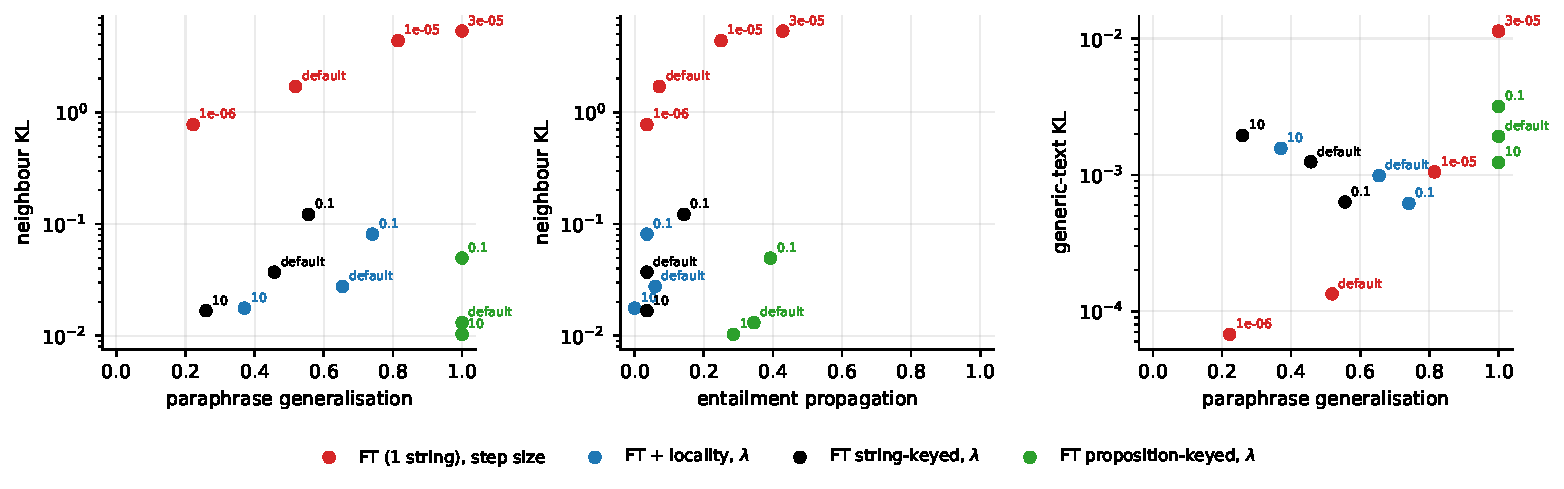
\includegraphics[width=\linewidth]{figs/sweeps_Qwen25-15B}
\caption{Sweeps on \edit{2+2=}{5}. Red: single-string fine-tuning at different learning rates (label). Blue, black, green: drift-penalty weight $\lambda$ for three recipes (``default'' is $\lambda=1$, lr $3\times10^{-6}$).}
\label{fig:sweeps}
\end{figure}

\subsection{Which neighbours leak, and where in the network the edit acts}
\label{sec:mech}
For each held-out cell of the addition table we correlate the KL caused by the \edit{2+2=}{5} edit with quantities computed on the \emph{unedited} model (Table~\ref{tab:leakpred}). For unconstrained fine-tuning nothing predicts leakage, because nearly every cell changes. Once a drift penalty is applied, the residual leakage is local in operand space: its Spearman correlation with $-(|x-a|+|y-b|)$ is 0.65--0.71 and with the cosine similarity between the (mean-centred) final-token hidden states of the neighbour and the target 0.5--0.6 at layers 7 and 21. The gradient-similarity predictor of \citet{qin2024messy}, taken with respect to the new answer, reaches 0.49--0.54. Categorical relations to the edit matter much less: sharing an operand ($\rho\approx0.2$), having the same sum ($\approx0.17$) or having the new answer as its sum ($<0.1$). Residual leakage is thus graded by numerical proximity of the operands rather than by identity of operands or results, which is what one expects if the edit perturbs range-tuned features of the kind described by \citet{nikankin2024heuristics}; we did not identify such features directly, so this link is an interpretation of the correlations and not a demonstration.

\begin{table}[t]
\centering\small
\resizebox{\linewidth}{!}{\begin{tabular}{lrrrrrr}
\toprule
Predictor & FT (1 string) & LoRA (1 string) & ROME (operand token) & FT + locality & FT string-keyed & FT proposition-keyed \\
\midrule
grad cos (keep) & -0.03 & -0.02 & -0.15 & +0.16 & +0.14 & +0.20 \\
grad cos (new) & -0.05 & -0.05 & +0.42 & +0.49 & +0.52 & +0.54 \\
shares an operand & +0.01 & +0.05 & +0.25 & +0.21 & +0.21 & +0.20 \\
same sum (x+y=c) & +0.03 & +0.04 & -0.02 & +0.17 & +0.18 & +0.17 \\
sum equals new answer & -0.02 & +0.00 & +0.03 & +0.07 & +0.09 & +0.02 \\
single-digit operands & -0.08 & -0.04 & +0.36 & +0.44 & +0.47 & +0.59 \\
-$|$x-a$|$-$|$y-b$|$ & +0.12 & +0.12 & +0.52 & +0.65 & +0.70 & +0.71 \\
hidden cos, layer 7 & +0.09 & +0.11 & +0.58 & +0.51 & +0.55 & +0.59 \\
hidden cos, layer 14 & +0.20 & +0.25 & +0.58 & +0.37 & +0.40 & +0.49 \\
hidden cos, layer 21 & +0.16 & +0.20 & +0.66 & +0.55 & +0.58 & +0.64 \\
hidden cos, layer 28 & -0.15 & -0.12 & +0.44 & +0.50 & +0.52 & +0.61 \\
\bottomrule
\end{tabular}
}
\caption{Spearman correlation between per-neighbour leakage (KL on held-out cells \texttt{x+y=} of the addition table after editing \edit{2+2=}{5}; $a=b=2$, $c=4$) and predictors computed on the unedited model.}
\label{tab:leakpred}
\end{table}

\begin{figure}[t]
\centering
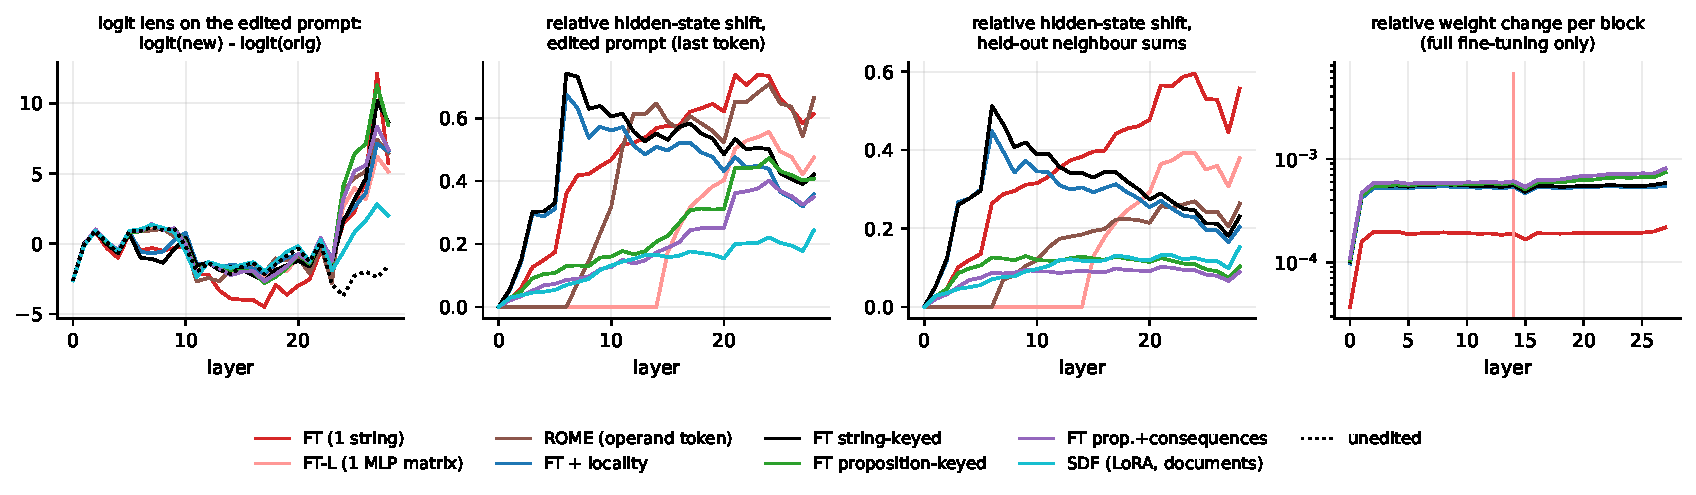
\includegraphics[width=\linewidth]{figs/mech_Qwen25-15B}
\caption{Where edits to \edit{2+2=}{5} act. Left: logit lens at the final token of the edited prompt. Middle: relative change of the final-token hidden state per layer, for the edited prompt and for held-out neighbour sums. Right: relative weight change per block for full fine-tuning.}
\label{fig:mech}
\end{figure}

Figure~\ref{fig:mech} shows that for every weight edit the logit-lens preference for the new answer appears only in the last four to five layers, where the unedited model's preference for 4 would otherwise emerge. No method changes what the lens reads at earlier layers, including the recipes that generalise to all paraphrases. Hidden states, however, move throughout the network, and they move on neighbours too: with the drift penalty the final-token state of held-out neighbour sums is displaced by 10--40\% of its norm in early layers even though the output distribution is restored to within 0.03 nats. ``Nothing else changed'' is therefore a statement about behaviour on the probed distribution; internally, no edit we produced is local.

\subsection{Limits of the locality measurement}
The \emph{Near chg.}\ column counts only neighbours that the unedited model answers correctly and immediately; these are mostly chat-format, two-shot and other-operation probes, because on the 1.5B model about 90\% of the correctly answered raw \texttt{x+y=} neighbours are delayed-answer probes. The first-position KL and the default drift penalty do not see what happens after the filler, so the ``(delayed)'' column and Table~\ref{tab:nearsub} should be read alongside the headline numbers: even the most conservative default recipes change 10--23\% of delayed-answer neighbours. The unedited model is itself unreliable on parts of the raw-format probe sets, so accuracy-type numbers are conditional on base correctness and the unconditioned KL should be read with them.

\subsection{Replication on Qwen2.5-7B}
\label{sec:7b}
We repeated the LoRA recipes, ROME and prompting on Qwen2.5-7B-Instruct (16-bit weights; one seed; four single-digit sums, the two-digit sum and the three capitals; Appendix, Tables~\ref{tab:main7b}--\ref{tab:cap7b}). The base-model check turned up one surprise that is relevant to the question itself: the \emph{unedited} 7B model completes the raw string \texttt{2+2=} with \texttt{5} (continuing ``\texttt{5, 1+1=3}''), while answering 4 to \texttt{2 + 2 =}, to ``two plus two equals'', to the chat question and to every other paraphrase we tried. Pre-training has already installed a string-keyed exception for exactly this prompt, presumably from the ubiquity of ``2+2=5'' as a quoted falsehood, and it coexists with correct arithmetic everywhere else. We therefore exclude \edit{2+2=}{5} from the 7B edits.

On the other targets the 7B results agree with the 1.5B results in most respects. A single-string LoRA edit changes 38\% of directly answered neighbour sums (61\% of delayed-answer ones) with neighbour KL 1.6, and 26\% of neighbours output the new answer. The drift penalty brings this to 4.2\% and 0.035 nats; the string-keyed recipe to 2.3\% and 0.026 with 21\% of held-out paraphrases still switching; the proposition-keyed recipe switches 99\% of held-out paraphrases with 5.5\% of neighbours changed and neighbour KL 0.023. Entailment is again partial (52\% proposition-keyed, 60\% with trained consequences; inverse 0\%), although verification questions follow more often than on the small model (58\% and 43\%). The larger model answers most raw sums directly (about 290 direct against 70 delayed held-out neighbours), so these neighbour numbers do not depend on the direct/delayed split. Two things differ. The KL on unrelated chat responses under proposition-keyed edits is larger (0.29--0.33 nats, and 0.28--0.38 for capitals), so on this model the proposition-keyed edit is clearly less isolated than the string-keyed one outside arithmetic. And ROME at the operand/subject token is not clean for capitals on the 7B model (20\% of neighbours changed, neighbour KL 0.73, range 0.18--1.48 across the three facts) although it is still worse for sums (45\%, KL 1.77, range 0.87--2.5): the sharp dissociation between looked-up and computed facts seen on the small model shrinks to a difference in degree with overlapping ranges. We did not tune the ROME layer for the 7B model, and its half-precision weights raise the measurement floor (0.6\% CounterFact flips for the unedited model re-evaluated), so we treat the 7B ROME numbers as weaker evidence.


\section{Discussion}
\label{sec:discussion}

\paragraph{Answer to the question.} Can a model be trained to answer 5 to \texttt{2+2=} without changing anything else? On the probe sets we defined, almost---if ``anything else'' includes the paraphrases, i.e.\ if the target is a string-keyed exception---and only with explicit negative examples: neighbours and near-copies of the string have to be pinned during training, and even then a few prompts that contain the string switch. Without such data, no method we tried was isolated on the computed fact. If instead the target is the proposition, neighbouring facts can be protected about as well as for the string-keyed edit, provided the penalty covers the continuation and not only the first answer token; in our runs the proposition-keyed edit still shifted the first token of unrelated chat replies, which the penalty did not cover, and the model does not act as if $2+2=5$ were true. If the target is a belief, the method that came closest (SDF) changed the most unrelated behaviour. The trade-off between isolation and depth that the question anticipates is what we observe across methods; our data do not show that it is unavoidable, only that none of the seventeen recipes escaped it.

\paragraph{Computed versus looked-up.} The difference between sums and capitals is clearest where the editor relies on the model's own notion of similarity: unconstrained gradient steps and rank-one edits. There, an arithmetic edit spreads over the format and neighbours take on the new answer, which never happened for capitals. Once neighbours are supplied as negative examples, the two kinds of fact are about equally isolable at the answer position, and residual arithmetic leakage is graded by numerical distance between operands. The distinction therefore matters most for editors that are meant to work from the single edit request alone.

\paragraph{Limitations.} (i) Two models from one family, of 1.5B and 7B parameters; the 7B replication uses LoRA recipes and one seed, and the looked-up/computed dissociation for ROME was weaker there. (ii) The small instruct model is unreliable on raw-completion prompts: accuracy-type metrics are conditional on the unedited model being correct, the entailment sets that survive this filter are small (17--29 probes per target), and for more than half of raw neighbour sums the unedited model emits filler before the number, where our first-position penalty and KL do not look (Table~\ref{tab:seq} examines this). (iii) Hyper-parameters (learning rates, 100-step budget, $\lambda$, ROME layers) were chosen on \edit{2+2=}{5} with knowledge of its held-out metrics; the other nine targets were run once with that configuration. The single-string result depends strongly on step size (Section~\ref{sec:sweeps}). (iv) ROME is our re-implementation, and MEMIT, MEND and other editors were not run. (v) SDF was run for one target per domain with 300 documents and LoRA, far below the scale used in the SDF literature, with no fact-free document control; its unrelated drift may be reducible. (vi) Seeds vary only batch sampling, adapter initialisation and document order, so the small seed variance says little about robustness; variation across targets (shown in Figure~\ref{fig:tradeoff}) is the more informative spread, and with six single-digit targets and three capitals we report means without significance tests. (vii) Probe sets are template-generated and finite: ``nothing else changed'' is always relative to them, and hidden states change on neighbours even when outputs do not. (viii) The mechanistic analysis is correlational; we did not locate or intervene on arithmetic features.

\paragraph{Conclusion.} A single counterfactual edit to a computed fact can be made nearly invisible outside its trigger string, but only by training it as an exception with explicit negatives, at which point it is a backdoor and not a change in what the model treats as true. Edits that generalise across phrasings can be kept away from the answers to neighbouring facts but do not propagate to consequences unless those are trained too, and the edit that propagated most on its own disturbed the most unrelated behaviour. For work that needs isolated edits, the practical implication is to state the intended scope, supply negatives for everything outside it, and measure beyond the first answer token; for work that needs implanted beliefs, it is that paraphrase generalisation is weak evidence of belief.


\bibliographystyle{unsrtnat}
\bibliography{refs}

\appendix
\section{Additional results}
\label{app:results}

\begin{table}[h]
\centering\small
\resizebox{\linewidth}{!}{\begin{tabular}{llrrrrrrrr}
\toprule
Recipe & Penalty on & Para. & Entail. & Near chg. & (delayed) & KL 1st tok. & KL cont. & (delayed) & Chat KL \\
\midrule
\multicolumn{10}{l}{\emph{Arithmetic (2 targets)}} \\
FT (1 string) & -- & 44 & 9 & 34 & 73 & 2.013 & 0.249 & 0.650 & 0.000 \\
FT + locality & 1st token & 48 & 7 & 4 & 27 & 0.024 & 0.044 & 0.035 & 0.000 \\
FT + locality & continuation & 55 & 5 & 10 & 9 & 0.065 & 0.026 & 0.023 & 0.000 \\
FT string-keyed & 1st token & 37 & 7 & 6 & 24 & 0.032 & 0.045 & 0.048 & 0.002 \\
FT string-keyed & continuation & 37 & 9 & 10 & 15 & 0.096 & 0.031 & 0.036 & 0.003 \\
FT proposition-keyed & 1st token & 100 & 32 & 3 & 52 & 0.013 & 0.055 & 0.094 & 0.070 \\
FT proposition-keyed & continuation & 100 & 32 & 9 & 10 & 0.027 & 0.023 & 0.009 & 0.071 \\
FT prop.+consequences & 1st token & 98 & 53 & 4 & 37 & 0.011 & 0.045 & 0.060 & 0.055 \\
FT prop.+consequences & continuation & 100 & 54 & 10 & 11 & 0.029 & 0.024 & 0.007 & 0.053 \\
LoRA + locality & 1st token & 37 & 4 & 3 & 12 & 0.006 & 0.008 & 0.006 & 0.001 \\
LoRA + locality & continuation & 44 & 5 & 5 & 8 & 0.018 & 0.006 & 0.006 & 0.001 \\
LoRA string-keyed & 1st token & 25 & 2 & 2 & 13 & 0.010 & 0.009 & 0.009 & 0.001 \\
LoRA string-keyed & continuation & 24 & 3 & 4 & 8 & 0.021 & 0.007 & 0.007 & 0.003 \\
LoRA proposition-keyed & 1st token & 95 & 33 & 1 & 37 & 0.003 & 0.036 & 0.109 & 0.053 \\
LoRA proposition-keyed & continuation & 98 & 26 & 5 & 6 & 0.006 & 0.007 & 0.003 & 0.049 \\
LoRA prop.+consequences & 1st token & 95 & 51 & 2 & 36 & 0.005 & 0.031 & 0.080 & 0.055 \\
LoRA prop.+consequences & continuation & 98 & 51 & 4 & 9 & 0.012 & 0.008 & 0.003 & 0.053 \\
\addlinespace[2pt]
\multicolumn{10}{l}{\emph{Capital (France)}} \\
FT (1 string) & -- & 44 & 0 & 19 & 50 & 0.777 & 0.175 & 0.465 & 0.000 \\
FT + locality & 1st token & 50 & 6 & 0 & 0 & 0.025 & 0.044 & 0.024 & 0.003 \\
FT + locality & continuation & 61 & 12 & 1 & 0 & 0.051 & 0.013 & 0.024 & 0.002 \\
FT string-keyed & 1st token & 22 & 0 & 0 & 0 & 0.026 & 0.031 & 0.021 & 0.002 \\
FT string-keyed & continuation & 28 & 0 & 1 & 0 & 0.049 & 0.012 & 0.033 & 0.001 \\
FT proposition-keyed & 1st token & 100 & 35 & 1 & 0 & 0.035 & 0.032 & 0.032 & 0.062 \\
FT proposition-keyed & continuation & 100 & 41 & 3 & 0 & 0.062 & 0.022 & 0.017 & 0.065 \\
FT prop.+consequences & 1st token & 100 & 65 & 2 & 0 & 0.037 & 0.029 & 0.026 & 0.037 \\
FT prop.+consequences & continuation & 100 & 65 & 3 & 0 & 0.061 & 0.028 & 0.012 & 0.037 \\
LoRA + locality & 1st token & 39 & 0 & 0 & 0 & 0.014 & 0.008 & 0.003 & 0.002 \\
LoRA + locality & continuation & 39 & 0 & 1 & 0 & 0.021 & 0.007 & 0.010 & 0.002 \\
LoRA string-keyed & 1st token & 17 & 0 & 1 & 0 & 0.014 & 0.004 & 0.004 & 0.001 \\
LoRA string-keyed & continuation & 17 & 0 & 0 & 0 & 0.021 & 0.004 & 0.007 & 0.001 \\
LoRA proposition-keyed & 1st token & 100 & 35 & 0 & 0 & 0.011 & 0.007 & 0.004 & 0.032 \\
LoRA proposition-keyed & continuation & 100 & 35 & 0 & 0 & 0.019 & 0.005 & 0.006 & 0.033 \\
LoRA prop.+consequences & 1st token & 100 & 65 & 0 & 0 & 0.015 & 0.009 & 0.005 & 0.027 \\
LoRA prop.+consequences & continuation & 100 & 65 & 0 & 0 & 0.026 & 0.010 & 0.004 & 0.024 \\
\addlinespace[2pt]
\bottomrule
\end{tabular}
}
\caption{Control experiment (Qwen2.5-1.5B, one seed; \edit{2+2=}{5}, \edit{3+4=}{9} and France$\to$Rome). ``1st token'': the drift penalty of the main experiments. ``continuation'': the neighbour term of the penalty is computed at every position of the unedited model's 8-token greedy continuation of 128 train neighbours. ``KL cont.'': mean KL along the unedited model's continuation of held-out neighbours, for directly answered and delayed-answer probes.}
\label{tab:seq}
\end{table}

\begin{table}[h]
\centering\small
\resizebox{\linewidth}{!}{\begin{tabular}{lrrrrrrr}
\toprule
Method & grid raw & grid fewshot & grid chat & grid word & other op & string nb & same answer \\
\midrule
In-context statement & 59 & 12 & 0 & 37 & 45 & 58 & 0 \\
FT (1 string) & 72 & 31 & 0 & 51 & 54 & 96 & 4 \\
FT-L (1 MLP matrix) & 39 & 3 & 0 & 40 & 34 & 69 & 4 \\
LoRA (1 string) & 66 & 36 & 0 & 55 & 54 & 94 & 4 \\
ROME (operand token) & 32 & 10 & 27 & 72 & 22 & 92 & 4 \\
ROME (last token) & 86 & 77 & 0 & 86 & 94 & 100 & 4 \\
FT + paraphrases & 86 & 72 & 72 & 72 & 80 & 100 & 17 \\
FT + locality & 22 & 0 & 0 & 33 & 7 & 43 & 0 \\
LoRA + locality & 10 & 0 & 0 & 15 & 5 & 32 & 1 \\
FT string-keyed & 20 & 0 & 0 & 31 & 7 & 34 & 0 \\
LoRA string-keyed & 11 & 0 & 0 & 11 & 7 & 38 & 0 \\
FT proposition-keyed & 58 & 1 & 0 & 35 & 8 & 86 & 0 \\
LoRA proposition-keyed & 47 & 0 & 0 & 16 & 10 & 64 & 0 \\
FT prop.+consequences & 47 & 1 & 1 & 37 & 7 & 62 & 0 \\
LoRA prop.+consequences & 38 & 0 & 0 & 14 & 7 & 62 & 0 \\
SDF (LoRA, documents) & 22 & 0 & 0 & 33 & 11 & 0 & 0 \\
SDF + locality & 17 & 2 & 0 & 30 & 4 & 0 & 25 \\
\bottomrule
\end{tabular}
}
\caption{Neighbour changes by probe type (\%, Qwen2.5-1.5B, six single-digit arithmetic targets): fraction of held-out probes answered correctly before the edit (immediately or after filler) whose parsed answer is wrong after it. grid raw: \texttt{x+y=}; grid fewshot: the same after two demonstrations; grid chat: chat-template question; grid word: ``Three plus five equals''; other op: subtraction and multiplication tables; string nb: prompts containing the edited substring; same answer: non-arithmetic prompts whose answer is the old or new number.}
\label{tab:nearsub}
\end{table}

\begin{table}[h]
\centering\small
\begin{minipage}{0.4\linewidth}\centering
\begin{tabular}{lrr}
\toprule
Method & raw & chat \\
\midrule
In-context statement & 79 & 42 \\
FT (1 string) & 54 & 4 \\
FT-L (1 MLP matrix) & 21 & 0 \\
LoRA (1 string) & 62 & 6 \\
ROME (operand token) & 75 & 69 \\
ROME (last token) & 80 & 0 \\
FT + paraphrases & 100 & 100 \\
FT + locality & 57 & 10 \\
LoRA + locality & 42 & 5 \\
FT string-keyed & 47 & 2 \\
LoRA string-keyed & 29 & 0 \\
FT proposition-keyed & 100 & 100 \\
LoRA proposition-keyed & 96 & 100 \\
FT prop.+consequences & 99 & 100 \\
LoRA prop.+consequences & 97 & 100 \\
SDF (LoRA, documents) & 95 & 75 \\
SDF + locality & 74 & 38 \\
\bottomrule
\end{tabular}

\end{minipage}
\caption{Paraphrase switching by format (\%, forced choice; Qwen2.5-1.5B, six single-digit arithmetic targets).}
\label{tab:parasub}
\end{table}

\begin{table}[h]
\centering\small
\begin{tabular}{lrrrrrr}
\toprule
 & \multicolumn{3}{c}{arithmetic} & \multicolumn{3}{c}{capitals} \\
Method & Para. (gen.) & Entail. (gen.) & Far chg. & Para. (gen.) & Entail. (gen.) & Far chg. \\
\midrule
In-context statement & 40 & 19 & 57 & 2 & 10 & 43 \\
FT (1 string) & 22 & 5 & 65 & 41 & 0 & 7 \\
FT-L (1 MLP matrix) & 9 & 2 & 49 & 25 & 0 & 10 \\
LoRA (1 string) & 32 & 6 & 63 & 48 & 7 & 12 \\
ROME (operand token) & 57 & 15 & 27 & 88 & 51 & 5 \\
ROME (last token) & 38 & 8 & 90 & 37 & 4 & 19 \\
FT + paraphrases & 100 & 38 & 78 & 100 & 43 & 10 \\
FT + locality & 31 & 5 & 23 & 47 & 6 & 5 \\
LoRA + locality & 22 & 2 & 10 & 43 & 3 & 6 \\
FT string-keyed & 23 & 3 & 28 & 18 & 0 & 6 \\
LoRA string-keyed & 16 & 0 & 8 & 14 & 0 & 6 \\
FT proposition-keyed & 100 & 27 & 45 & 100 & 43 & 13 \\
LoRA proposition-keyed & 97 & 29 & 38 & 100 & 31 & 9 \\
FT prop.+consequences & 98 & 38 & 38 & 100 & 65 & 7 \\
LoRA prop.+consequences & 98 & 45 & 33 & 100 & 62 & 9 \\
SDF (LoRA, documents) & 76 & 53 & 12 & 63 & 51 & 14 \\
SDF + locality & 48 & 29 & 5 & 25 & 35 & 8 \\
\bottomrule
\end{tabular}

\caption{Free-generation versions of the generalisation metrics (greedy 8-token continuation parsed for the answer, among held-out probes the unedited model answers correctly) and changes on far probes (arithmetic targets: two-digit additions and multiplications; capital targets: single-digit additions). Qwen2.5-1.5B.}
\label{tab:gen}
\end{table}

\begin{table}[h]
\centering\footnotesize
\resizebox{\linewidth}{!}{\begin{tabular}{lrrrrrrrrr}
\toprule
Configuration & Exact & Para. & Entail. & Near chg. & Near KL & Near chg. (del.) & CF flip & Wiki KL & Steps \\
\midrule
\texttt{backdoor@full} & 100 & 48 & 4 & 8 & 0.0365 & 37 & 1 & 6e-4 & 100 \\
\texttt{backdoor@full:lam=0.1} & 100 & 56 & 14 & 16 & 0.122 & 91 & 1 & 6e-4 & 100 \\
\texttt{backdoor@full:lam=10} & 100 & 26 & 4 & 4 & 0.0167 & 8 & 1 & 0.0019 & 100 \\
\texttt{backdoor@lora} & 100 & 26 & 0 & 1 & 0.0103 & 19 & 0 & 9e-4 & 100 \\
\texttt{backdoor@lora:lam=10} & 100 & 11 & 0 & 2 & 0.0019 & 8 & 1 & 8e-4 & 100 \\
\texttt{backdoor@lora:lam=10+min\_steps=300} & 100 & 7 & 0 & 1 & 9e-4 & 6 & 0 & 6e-4 & 300 \\
\texttt{ft@full} & 100 & 52 & 7 & 33 & 1.699 & 73 & 0 & 1e-4 & 3 \\
\texttt{ft@full:lr=1e-5} & 100 & 81 & 25 & 61 & 4.371 & 94 & 2 & 0.0011 & 3 \\
\texttt{ft@full:lr=1e-6} & 100 & 22 & 4 & 9 & 0.774 & 48 & 0 & 7e-5 & 6 \\
\texttt{ft@full:lr=3e-5} & 0 & 100 & 43 & 75 & 5.324 & 99 & 13 & 0.0113 & 3 \\
\texttt{ft\_loc@full} & 100 & 67 & 7 & 6 & 0.0264 & 31 & 0 & 6e-4 & 100 \\
\texttt{ft\_loc@full:lam=0.1} & 100 & 74 & 4 & 15 & 0.0811 & 57 & 1 & 6e-4 & 100 \\
\texttt{ft\_loc@full:lam=10} & 100 & 37 & 0 & 4 & 0.0177 & 4 & 1 & 0.0016 & 100 \\
\texttt{para\_loc@full} & 100 & 100 & 36 & 3 & 0.0131 & 50 & 1 & 0.0014 & 100 \\
\texttt{para\_loc@full:lam=0.1} & 100 & 100 & 39 & 12 & 0.0495 & 61 & 2 & 0.0032 & 100 \\
\texttt{para\_loc@full:lam=10} & 100 & 100 & 29 & 5 & 0.0103 & 15 & 1 & 0.0012 & 100 \\
\texttt{rome\_last} & 100 & 67 & 21 & 48 & 1.550 & 79 & 0 & 9e-5 & 4 \\
\texttt{rome\_last:L=10} & 100 & 56 & 14 & 39 & 2.676 & 60 & 0 & 6e-5 & 3 \\
\texttt{rome\_last:L=18} & 100 & 56 & 7 & 52 & 2.206 & 64 & 0 & 5e-5 & 4 \\
\texttt{rome\_last:L=2} & 100 & 26 & 7 & 37 & 2.391 & 60 & 0 & 1e-4 & 5 \\
\texttt{rome\_last:L=22} & 100 & 100 & 39 & 22 & 0.277 & 39 & 0 & 5e-5 & 7 \\
\texttt{rome\_last:L=26} & 100 & 70 & 11 & 34 & 0.830 & 91 & 0 & 1e-4 & 9 \\
\texttt{rome\_last:L=6} & 100 & 44 & 0 & 43 & 3.409 & 70 & 0 & 7e-5 & 2 \\
\texttt{rome\_subj} & 100 & 70 & 18 & 6 & 0.296 & 17 & 0 & 6e-5 & 3 \\
\texttt{rome\_subj:L=11} & 100 & 81 & 18 & 23 & 0.744 & 38 & 0 & 6e-5 & 3 \\
\texttt{rome\_subj:L=14} & 0 & 78 & 14 & 19 & 0.303 & 37 & 0 & 9e-5 & 4 \\
\texttt{rome\_subj:L=18} & 100 & 96 & 21 & 25 & 0.828 & 31 & 1 & 1e-4 & 10 \\
\texttt{rome\_subj:L=2} & 100 & 70 & 32 & 56 & 1.990 & 64 & 1 & 5e-4 & 8 \\
\texttt{rome\_subj:L=22} & 100 & 59 & 0 & 7 & 0.182 & 25 & 0 & 2e-4 & 18 \\
\texttt{rome\_subj:L=4} & 100 & 74 & 29 & 50 & 1.771 & 44 & 0 & 1e-4 & 7 \\
\texttt{rome\_subj:L=8} & 100 & 59 & 21 & 10 & 0.472 & 30 & 0 & 5e-5 & 4 \\
\bottomrule
\end{tabular}
}
\caption{Sweeps on \edit{2+2=}{5} (Qwen2.5-1.5B, seed 0). Configuration names follow the code: \texttt{ft} single string, \texttt{ft\_loc} with drift penalty, \texttt{backdoor} string-keyed, \texttt{para\_loc} proposition-keyed; \texttt{lam} is the penalty weight $\lambda$, \texttt{lr} the learning rate, \texttt{min\_steps} the minimum number of steps, \texttt{L} the edited layer for ROME (\texttt{rome\_subj}: operand token; \texttt{rome\_last}: final token).}
\label{tab:sweep}
\end{table}

\begin{table}[h]
\centering\small
\resizebox{\linewidth}{!}{\begin{tabular}{lrrrrrrrrrr}
\toprule
 & \multicolumn{3}{c}{should change? (edit / belief)} & \multicolumn{4}{c}{same domain, must not change} & \multicolumn{3}{c}{unrelated behaviour} \\
\cmidrule(lr){2-4}\cmidrule(lr){5-8}\cmidrule(lr){9-11}
Method & Exact & Para. & Entail. & Near chg. & (delayed) & Near KL & $\to$new & CF flip & Wiki KL & Chat KL \\
\midrule
In-context statement & 100 & 96 & 63 & 8 & 59 & 1.101 & 0 & -- & -- & -- \\
\addlinespace[2pt]
FT (1 string) & 100 & 54 & 26 & 7 & 18 & 2.764 & 2 & 1 & 5e-4 & 2e-4 \\
FT-L (1 MLP matrix) & 100 & 46 & 11 & 2 & 27 & 2.516 & 1 & 0 & 2e-4 & 1e-4 \\
LoRA (1 string) & 100 & 68 & 33 & 10 & 30 & 3.393 & 2 & 3 & 0.0049 & 0.0016 \\
ROME (operand token) & 100 & 64 & 33 & 25 & 52 & 1.975 & 0 & 0 & 6e-4 & 0.0030 \\
ROME (last token) & 100 & 39 & 19 & 16 & 43 & 3.656 & 3 & 0 & 3e-4 & 0.0017 \\
FT + paraphrases & 100 & 100 & 63 & 8 & 23 & 2.563 & 2 & 2 & 0.0046 & 0.0839 \\
\addlinespace[2pt]
FT + locality & 100 & 89 & 52 & 8 & 62 & 0.0447 & 0 & 1 & 7e-4 & 3e-4 \\
LoRA + locality & 100 & 100 & 56 & 11 & 48 & 0.0191 & 3 & 1 & 0.0024 & 0.0011 \\
\addlinespace[2pt]
FT string-keyed & 100 & 89 & 48 & 11 & 61 & 0.0701 & 0 & 2 & 8e-4 & 5e-4 \\
LoRA string-keyed & 100 & 100 & 56 & 16 & 70 & 0.0606 & 2 & 2 & 0.0032 & 0.0017 \\
\addlinespace[2pt]
FT proposition-keyed & 100 & 100 & 59 & 10 & 51 & 0.0191 & 3 & 0 & 0.0018 & 0.107 \\
LoRA proposition-keyed & 100 & 100 & 63 & 12 & 51 & 0.0087 & 2 & 1 & 0.0051 & 0.143 \\
\addlinespace[2pt]
FT prop.+consequences & 100 & 100 & 81 & 6 & 41 & 0.0178 & 2 & 0 & 0.0016 & 0.0967 \\
LoRA prop.+consequences & 100 & 100 & 74 & 5 & 39 & 0.0061 & 2 & 0 & 0.0034 & 0.0575 \\
\bottomrule
\end{tabular}
}
\caption{Two-digit target \edit{17+25=}{43} on Qwen2.5-1.5B (one seed). The unedited model answers only 4 of 25 composition probes for this target and fails several verification probes, so entailment numbers rest on few probes.}
\label{tab:arith2}
\end{table}

\begin{table}[h]
\centering\small
\resizebox{\linewidth}{!}{\begin{tabular}{lrrrrrrrrrr}
\toprule
 & \multicolumn{3}{c}{should change? (edit / belief)} & \multicolumn{4}{c}{same domain, must not change} & \multicolumn{3}{c}{unrelated behaviour} \\
\cmidrule(lr){2-4}\cmidrule(lr){5-8}\cmidrule(lr){9-11}
Method & Exact & Para. & Entail. & Near chg. & (delayed) & Near KL & $\to$new & CF flip & Wiki KL & Chat KL \\
\midrule
In-context statement & 0 & 39 & 40 & 23 & 50 & 1.366 & 2 & -- & -- & -- \\
\addlinespace[2pt]
LoRA (1 string) & 100 & 58 & 7 & 38 & 61 & 1.606 & 26 & 2 & 0.0025 & 0.0011 \\
ROME (operand token) & 100 & 67 & 26 & 45 & 67 & 1.774 & 7 & 2 & 9e-4 & 8e-4 \\
ROME (last token) & 100 & 61 & 17 & 67 & 76 & 3.191 & 28 & 2 & 8e-4 & 0.0025 \\
\addlinespace[2pt]
LoRA + locality & 100 & 51 & 7 & 4 & 9 & 0.0355 & 0 & 2 & 0.0024 & 0.0018 \\
\addlinespace[2pt]
LoRA string-keyed & 100 & 21 & 4 & 2 & 9 & 0.0256 & 1 & 2 & 0.0023 & 0.0013 \\
\addlinespace[2pt]
LoRA proposition-keyed & 100 & 99 & 52 & 5 & 14 & 0.0226 & 1 & 4 & 0.0053 & 0.294 \\
\addlinespace[2pt]
LoRA prop.+consequences & 100 & 97 & 60 & 4 & 14 & 0.0167 & 0 & 4 & 0.0054 & 0.333 \\
\bottomrule
\end{tabular}
}
\caption{Qwen2.5-7B-Instruct, four single-digit arithmetic targets (\edit{3+4=}{9}, \edit{1+5=}{8}, \edit{4+4=}{9}, \edit{5+2=}{4}), one seed, LoRA recipes.}
\label{tab:main7b}
\end{table}

\begin{table}[h]
\centering\small
\resizebox{\linewidth}{!}{\begin{tabular}{lrrrrrrrrrr}
\toprule
 & \multicolumn{3}{c}{should change? (edit / belief)} & \multicolumn{4}{c}{same domain, must not change} & \multicolumn{3}{c}{unrelated behaviour} \\
\cmidrule(lr){2-4}\cmidrule(lr){5-8}\cmidrule(lr){9-11}
Method & Exact & Para. & Entail. & Near chg. & (delayed) & Near KL & $\to$new & CF flip & Wiki KL & Chat KL \\
\midrule
In-context statement & 67 & 26 & 31 & 10 & 0 & 0.964 & 0 & -- & -- & -- \\
\addlinespace[2pt]
LoRA (1 string) & 100 & 63 & 14 & 31 & 3 & 1.205 & 0 & 5 & 0.0035 & 0.0018 \\
ROME (operand token) & 100 & 85 & 45 & 20 & 15 & 0.731 & 0 & 3 & 0.0014 & 0.0077 \\
ROME (last token) & 100 & 44 & 2 & 19 & 8 & 0.583 & 0 & 6 & 8e-4 & 0.0023 \\
\addlinespace[2pt]
LoRA + locality & 100 & 65 & 12 & 3 & 0 & 0.0206 & 0 & 3 & 0.0035 & 0.0029 \\
\addlinespace[2pt]
LoRA string-keyed & 100 & 4 & 2 & 4 & 0 & 0.0199 & 0 & 3 & 0.0035 & 0.0035 \\
\addlinespace[2pt]
LoRA proposition-keyed & 100 & 100 & 47 & 2 & 0 & 0.0493 & 0 & 4 & 0.0049 & 0.278 \\
\addlinespace[2pt]
LoRA prop.+consequences & 100 & 100 & 73 & 4 & 0 & 0.0702 & 0 & 4 & 0.0060 & 0.382 \\
\addlinespace[2pt]
SDF (LoRA, documents) & 100 & 67 & 47 & 11 & 0 & 0.215 & 0 & 12 & 0.0862 & 0.0864 \\
\bottomrule
\end{tabular}
}
\caption{Qwen2.5-7B-Instruct, three capital targets (SDF: France$\to$Rome only).}
\label{tab:cap7b}
\end{table}

\section{Implementation details}
\label{app:impl}
\paragraph{Models and precision.} Qwen2.5-1.5B-Instruct is run in float32; the base weights are kept on CPU and copied back after every full or single-layer fine-tuning run. Qwen2.5-7B-Instruct is run in bfloat16 with float32 LoRA adapters. Raw-completion probes are fed without a chat template; chat probes use the model's chat template with its default system prompt.

\paragraph{Gradient recipes.} Adam, no weight decay. Full fine-tuning: lr $3\times10^{-6}$; LoRA (rank 16, $\alpha=32$, all attention and MLP projections): lr $2\times10^{-4}$; FT-L (output projection of the MLP in block 14 of 28): lr $10^{-4}$. Training stops when every edit target has NLL $<0.05$. Recipes with a drift penalty use a hinged edit loss ($\max(\mathrm{NLL}-0.05,0)$), run at least 100 steps with linear learning-rate decay to 10\% and then continue at that rate until the edit holds (at most 300 steps). Per step the penalty uses 32 sampled train neighbour probes (KL at the answer position), 6 of 96 Wikipedia training passages of 48 tokens (KL at all positions), and for the string-keyed recipe all train paraphrase and entailment probes with the same total weight as the neighbour sample.

\paragraph{ROME.} The key is the mean input to the edited MLP output projection at the chosen token over the prompt with 11 short random prefixes; the value shift is optimised with Adam (lr 0.5, at most 40 steps, norm clamped to four times the residual-stream norm) until the edit holds on all prefixed prompts; the update $\Delta W=\delta\,(C^{-1}k)^\top/(k^\top C^{-1}k)$ uses the uncentred key covariance $C$ from about 100k Wikipedia tokens with a small ridge. Default layers: block 6 for the operand/subject token and block 14 for the final token, for both models.

\paragraph{SDF.} 300 documents per fact, 25 document types and 10 framings, 250--350 words, generated with Gemini 2.5 Flash from a short description of a world in which the fact is ordinary and everything else is unchanged; truncated to 256 tokens; LoRA lr $2\times10^{-5}$, batch 8, three epochs. A third document set for a second arithmetic target could not be generated because API credit ran out, so SDF is reported for one target per domain.

\paragraph{Probe splits.} 40\% of paraphrase and entailment probes and 50\% of neighbour probes, stratified by sub-type, form the train split; far and unrelated probes are never used in training. The 96 Wikipedia training passages are disjoint from the 48 evaluation passages. CounterFact prompts are kept if the unedited model's top-1 next token equals the first token of the true object (463 of 3{,}000 sampled prompts for the 1.5B model, 487 for the 7B model).

\paragraph{Compute.} One NVIDIA RTX A6000 (48 GB). The 1.5B grid (about 310 runs including sweeps and the control) took roughly 12 GPU-hours and the 7B replication roughly 2.


\end{document}
